\chapter[Nonlinear Least Squares and Optimization]{Nonlinear Least Squares\\ and Optimization}
\label{ch:nlls}
\chaptermark{Nonlinear Least Squares} % short running header

\begin{objectives}
\begin{itemize}
  \item Formulate estimation problems with nonlinear models as nonlinear least-squares problems.
  \item Derive Newton, Gauss--Newton and Levenberg--Marquardt iterations, and understand when each converges.
  \item Optimize over manifolds such as $\SO$ by iterating in the tangent space.
  \item Make least squares robust to outliers with M-estimators and iteratively reweighted least squares.
  \item Exploit the structure of problems with poses and landmarks: the Schur complement and marginalization.
  \item See that an extended Kalman update is one Gauss--Newton step, the bridge between filtering and optimization.
\end{itemize}
\end{objectives}

Most measurement models in VIO are nonlinear: projections divide by depth, rotations enter through trigonometric functions. Maximum
likelihood with Gaussian noise then becomes a \emph{nonlinear} least-squares problem with no closed-form solution. This chapter develops the
iterative methods that solve such problems. They are used directly in this project for triangulation, and they explain what the extended
Kalman filter and the MSCKF are doing.

% ==============================================================================
\section{The problem}

Given residual functions $r_i(x)$ (measurement minus prediction) with noise covariances $R_i$, the maximum-likelihood estimate minimizes
\begin{equation}
  F(x) = \frac12\sum_i r_i(x)\T R_i\inv r_i(x) = \frac12\,r(x)\T W\,r(x),
  \label{eq:nlls}
\end{equation}
where $r$ stacks the residuals and $W = \blkdiag(R_i\inv)$. Examples in these notes:
\begin{itemize}
  \item \emph{Triangulation}: find a 3D point minimizing the reprojection errors in several images (\cref{ch:multiview}).
  \item \emph{Relative pose}: find the motion between two images that best explains point correspondences.
  \item \emph{Bundle adjustment}: find all camera poses and all points at once.
  \item \emph{Sliding-window VIO}: find a window of states minimizing visual and inertial residuals together.
\end{itemize}
Writing $W = L\T L$ (for instance $L$ the inverse of a Cholesky factor of the noise covariance) and replacing $r$ by $Lr$ \emph{whitens} the residuals,
so that $W = I$. We do this silently when convenient.

% ==============================================================================
\section{Descent methods}

The gradient and Hessian of $F$ follow from the chain rule. With $J = \partial r/\partial x$,
\begin{equation}
  \nabla F = J\T Wr, \qquad \nabla^2F = J\T WJ + \sum_k(Wr)_k\,\nabla^2r_k .
  \label{eq:nlls-derivatives}
\end{equation}

\paragraph{Gradient descent.} Step downhill, $x \gets x - \alpha\nabla F$, with a step length $\alpha$ chosen by a line search. It always makes progress for small
enough $\alpha$, but it ignores curvature and zig-zags slowly along narrow valleys.

\paragraph{Newton's method.} Minimize the quadratic Taylor model $F(x + \delta) \approx F + \nabla F\T\delta + \tfrac12\delta\T\nabla^2F\,\delta$ exactly:
\begin{equation}
  \nabla^2F\,\delta = -\nabla F .
\end{equation}
Near a minimum with positive-definite Hessian, Newton's method converges \emph{quadratically}: the number of correct digits roughly doubles each
iteration. But it needs second derivatives of every residual, and far from the minimum the Hessian may not be positive definite, in which case the
step can go uphill.

% ==============================================================================
\section{Gauss--Newton}
\label{sec:gauss-newton}

\index{Gauss--Newton method}
Least-squares problems allow a better compromise. Linearize the \emph{residuals} rather than the cost: $r(x + \delta) \approx r + J\delta$. The cost then
becomes a linear least-squares problem in $\delta$,
\begin{equation}
  \min_\delta\ \tfrac12\|r + J\delta\|_W^2
  \quad\Longrightarrow\quad
  \big(J\T WJ\big)\,\delta = -J\T Wr,
  \label{eq:gn-step}
\end{equation}
the \term{Gauss--Newton} step. Comparing with \eqref{eq:nlls-derivatives}, Gauss--Newton is Newton's method with the second term of the Hessian dropped.
That term is small when the residuals are small at the solution, or when the residuals are nearly linear, which is the common case for
well-modeled sensors. Then Gauss--Newton converges almost as fast as Newton, without second derivatives. The approximate Hessian $J\T WJ$ is
always positive semi-definite, so the step is always a descent direction (if $J$ has full column rank).

\begin{algorithm}[h]
\caption{Gauss--Newton}
\label{alg:gauss-newton}
\begin{algorithmic}[1]
\Require initial guess $x$, residual function $r(x)$ and its Jacobian $J(x)$
\Repeat
  \State evaluate $r$ and $J$ at $x$
  \State solve $(J\T WJ)\,\delta = -J\T Wr$ \Comment{Cholesky of $J\T WJ$, or QR of the whitened $J$}
  \State $x \gets x + \delta$
\Until{$\|\delta\|$ or the decrease of $F$ is below a tolerance}
\end{algorithmic}
\end{algorithm}

The linear system is the normal equation of a linear least-squares problem, so all the numerical advice of \cref{sec:least-squares} applies: for
small, well-conditioned problems Cholesky of $J\T WJ$ is fine; for ill-conditioned ones, QR of the whitened Jacobian is safer.

\paragraph{When Gauss--Newton fails.} With a poor initial guess, large residuals or strong nonlinearity, the linear model can be a bad
approximation, and a full step can increase the cost. If $J\T WJ$ is singular, some direction is not determined by the data (a \emph{gauge freedom}
or an unobservable direction), and the step is undefined.

\section{Levenberg--Marquardt}

\index{Levenberg--Marquardt method}
The \term{Levenberg--Marquardt} (LM) method damps the Gauss--Newton step:
\begin{equation}
  \big(J\T WJ + \lambda D\big)\,\delta = -J\T Wr, \qquad \lambda \ge 0,
\end{equation}
with $D = I$ or $D = \diag(J\T WJ)$. For $\lambda\to0$ it is Gauss--Newton; for large $\lambda$ the step becomes a short gradient-descent step. The damping is
adapted to how well the linear model predicted the actual change of cost. With the \emph{gain ratio}
\begin{equation}
  \rho = \frac{F(x) - F(x + \delta)}{F(x) - \tfrac12\|r + J\delta\|_W^2},
\end{equation}
a step with $\rho$ close to one is accepted and $\lambda$ decreased (trust the model more), while a step with small or negative $\rho$ is rejected and
$\lambda$ increased. LM is equivalent to a \emph{trust-region} method that restricts the step to a region where the linearization is trusted. It is
the default solver of most computer-vision and robotics libraries.

\begin{figure}[t]
  \centering
  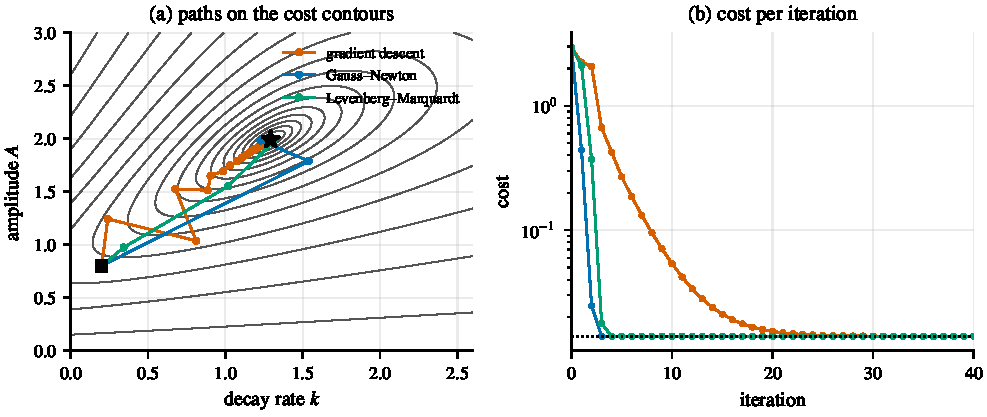
\includegraphics[width=\textwidth]{fig_gn_lm.pdf}
  \caption{Fitting the decay rate and amplitude of an exponential to noisy data. (a) Paths of gradient descent, Gauss--Newton and
  Levenberg--Marquardt on the contours of the cost, from the same starting point. (b) Cost versus iteration. Gradient descent crawls along the
  curved valley; Gauss--Newton and LM reach the minimum in a handful of iterations.}
  \label{fig:gn-lm}
\end{figure}

\section{Uncertainty of the solution}

At the minimum $\hat x$, the cost is approximately quadratic, $F(\hat x + \delta) \approx F(\hat x) + \tfrac12\delta\T(J\T WJ)\delta$, and with $W$ equal to the inverse
noise covariance the estimate has approximately the WLS covariance of the linearized problem (\cref{prop:wls-cov}):
\begin{equation}
  \Cov(\hat x) \approx \big(J\T WJ\big)\inv\Big|_{\hat x} .
\end{equation}
This is the \emph{Laplace approximation}: the posterior is replaced by a Gaussian fitted to its peak. It is accurate when the problem is nearly
linear over the region of uncertainty. A triangulated point, for example, gets a covariance from the Jacobians of its reprojection errors.

% ==============================================================================
\section{Optimization on manifolds}
\label{sec:manifold-opt}

When the unknown includes rotations, $x + \delta$ is replaced by the retraction $x\bplus\delta$ of \cref{ch:lie}. Linearize the residual in the tangent space,
$r(x\bplus\delta) \approx r(x) + J\delta$ with $J$ the manifold Jacobian (\cref{def:manifold-jacobian}), solve the same Gauss--Newton equation for $\delta$, and
update $x \gets x\bplus\delta$. The step is computed in a flat space and applied on the curved one, so the iterate never leaves the manifold and no
constraint ever needs enforcing. Covariances are then expressed in the tangent space at the solution, exactly as in a filter.

\begin{example}[Rotation averaging as Gauss--Newton]
Average rotations $R_1, \dots, R_N$ (\cref{ch:lie}) by minimizing $\tfrac12\sum_i\|r_i\|^2$ with $r_i(\bar R) = \Log(\bar R\T R_i)$. Perturbing
$\bar R\bplus\delta = \bar R\Exp(\delta)$ gives $r_i = \Log(\Exp(-\delta)\bar R\T R_i) \approx r_i(\bar R) - \Jlinv(r_i)\,\delta$ (\cref{eq:bch-left}). For small residuals
$\Jlinv \approx I$, so $J_i \approx -I$, and the Gauss--Newton step is $\delta = \frac1N\sum_ir_i$: exactly the averaging iteration of \cref{ch:lie}.
\end{example}

% ==============================================================================
\section{Robust estimation}
\label{sec:robust}

\subsection{Outliers break least squares}

A squared cost gives enormous influence to large residuals: a single wrong measurement, far from the others, can drag a least-squares estimate
arbitrarily far. Real data contain such \term{outliers}: misassociated features, reflections, moving objects. Two defenses exist: detect and
remove them (gating, RANSAC), or reduce their influence with a robust cost.

\subsection{M-estimators}

\index{M-estimator}\index{robust kernel}
An \term{M-estimator} replaces the quadratic by a function $\rho$ of the whitened residual norm $s_i = \|r_i\|_{R_i\inv}$:
\begin{equation}
  \min_x\ \sum_i\rho(s_i) .
\end{equation}

\begin{center}\small
\begin{tabular}{@{}l l l@{}}
\toprule
Kernel & $\rho(s)$ & weight $w(s) = \rho'(s)/s$ \\
\midrule
least squares & $\tfrac12s^2$ & $1$ \\
Huber & $\tfrac12s^2$ for $s\le c$;\ \ $c(s - \tfrac c2)$ otherwise & $1$ for $s \le c$;\ \ $c/s$ otherwise \\
Cauchy & $\tfrac{c^2}2\log(1 + s^2/c^2)$ & $1/(1 + s^2/c^2)$ \\
Tukey & $\tfrac{c^2}6\big(1 - (1 - s^2/c^2)^3\big)$ for $s \le c$;\ \ $c^2/6$ otherwise & $(1 - s^2/c^2)^2$ for $s \le c$;\ \ $0$ otherwise \\
\bottomrule
\end{tabular}
\end{center}

\begin{figure}[t]
  \centering
  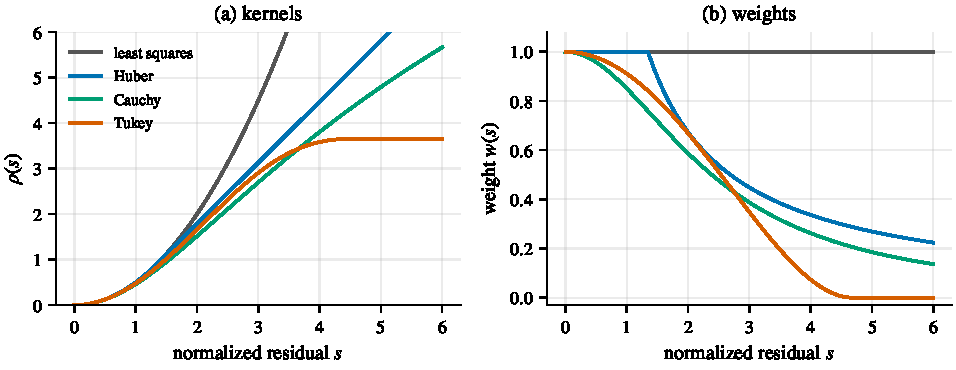
\includegraphics[width=\textwidth]{fig_robust_kernels.pdf}
  \caption{Robust kernels (left) and their weights (right) as functions of the normalized residual, for $c = 1.345$ (Huber), $2.385$ (Cauchy) and
  $4.685$ (Tukey). Huber grows linearly instead of quadratically for large residuals; Cauchy grows logarithmically; Tukey ignores residuals beyond
  $c$ entirely.}
  \label{fig:robust-kernels}
\end{figure}

The derivative $\psi = \rho'$ (the \emph{influence function}) measures how hard a residual pulls on the estimate: unbounded and linear for least squares,
bounded for Huber, decreasing to zero for Cauchy and Tukey (\cref{fig:robust-kernels}). The constants $c$ trade efficiency on clean Gaussian data against
robustness; the values in the figure keep 95\% of the efficiency of least squares on Gaussian noise.

\subsection{Iteratively reweighted least squares}

Setting the gradient of $\sum_i\rho(s_i)$ to zero gives $\sum_iw(s_i)J_i\T R_i\inv r_i = 0$ with $w(s) = \rho'(s)/s$: the normal equations of a \emph{weighted}
least-squares problem whose weights depend on the residuals. \emph{Iteratively reweighted least squares} (IRLS) alternates: compute the weights
from the current residuals, take a Gauss--Newton step with those weights, repeat. Outliers receive small weights and stop dominating. Robust
kernels need a reasonable initial guess, because with large initial errors every residual looks like an outlier; RANSAC (\cref{ch:multiview})
provides such guesses.

Gating, used in filters, is the hard-decision version of the same idea: a measurement whose normalized residual exceeds a threshold gets weight
zero, all others weight one, a ``truncated quadratic'' kernel.

% ==============================================================================
\section{Structure: poses, landmarks and the Schur complement}
\label{sec:schur-ba}

Many estimation problems have two kinds of unknowns. In bundle adjustment, the cameras $c$ and the landmarks $l$; in VIO smoothing, the states in
a window and the features. Each residual involves one camera and one landmark, so the normal equations have a special block structure:
\begin{equation}
  \begin{bmatrix} A & B \\ B\T & C \end{bmatrix}\begin{bmatrix}\delta c\\ \delta l\end{bmatrix} = \begin{bmatrix}g_c\\ g_l\end{bmatrix},
\end{equation}
where $C$, the landmark block of $J\T WJ$, is block diagonal with one $3\times3$ block per landmark (no residual involves two landmarks). Inverting $C$ is
therefore cheap. Eliminating the landmarks with the Schur complement (\cref{sec:schur}),
\begin{equation}
  \big(A - BC\inv B\T\big)\,\delta c = g_c - BC\inv g_l, \qquad \delta l = C\inv(g_l - B\T\delta c),
  \label{eq:reduced-camera-system}
\end{equation}
leaves a \emph{reduced camera system} whose size depends only on the number of cameras, often a hundred times smaller than the full problem.

\begin{figure}[t]
  \centering
  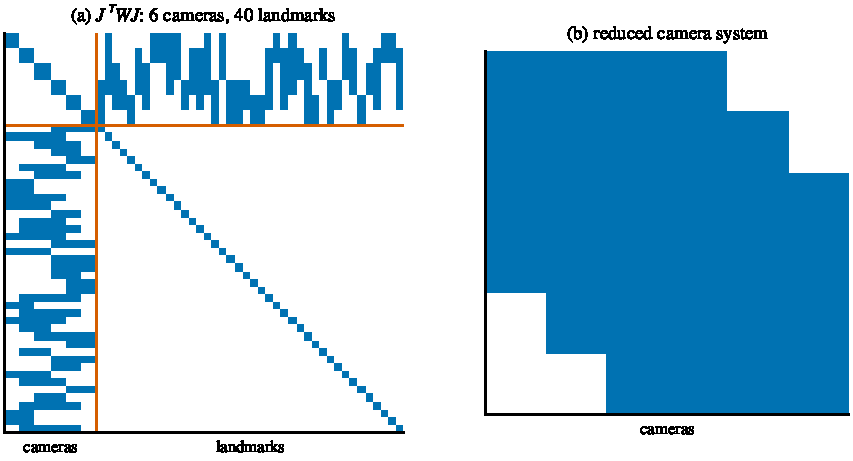
\includegraphics[width=\textwidth]{fig_ba_sparsity.pdf}
  \caption{Sparsity of the normal-equation matrix $J\T WJ$ for a toy bundle adjustment with 6 cameras and 40 landmarks (left), and of the reduced camera
  system after eliminating the landmarks (right). The landmark block is block-diagonal and cheap to eliminate; the reduced system is small but dense.}
  \label{fig:ba-sparsity}
\end{figure}

The same operation has a probabilistic meaning. $J\T WJ$ is the information matrix of the linearized problem, and the Schur complement is
\emph{marginalization in information form} (\cref{thm:gauss-cond}): the reduced system is the information that the measurements carry about the
cameras alone, after the landmarks have been integrated out. Sliding-window estimators use exactly this to discard old states, keeping their
information as a Gaussian prior on the remaining ones; the price is \emph{fill-in}, since the reduced matrix is dense (\cref{fig:ba-sparsity}). The
MSCKF performs the same elimination of each landmark, by a different algebraic route: the left-nullspace projection (\cref{ch:msckfupdate}).

% ==============================================================================
\section{Filtering as optimization}
\label{sec:filter-gn}

\begin{proposition}[The EKF update is one Gauss--Newton step]
\label{prop:ekf-gn}
\index{iterated EKF}
Consider the MAP cost of one measurement $z = h(x) + n$, $n \sim \N(0, R)$, with prior $\N(\mu, P)$:
\begin{equation*}
  F(x) = \tfrac12\|x - \mu\|^2_{P\inv} + \tfrac12\|z - h(x)\|^2_{R\inv}.
\end{equation*}
One Gauss--Newton step from $x = \mu$ gives $x^+ = \mu + K(z - h(\mu))$ with $K = PH\T(HPH\T + R)\inv$ and $H = \partial h/\partial x|_\mu$: the extended
Kalman update (\cref{ch:nonlinear}).
\end{proposition}
\begin{proof}
The stacked residual is $r(x) = \big(L_P(x - \mu),\ L_R(h(x) - z)\big)$ with $L_P\T L_P = P\inv$ and $L_R\T L_R = R\inv$. At $x = \mu$, $r = (0,\ L_R(h(\mu) - z))$ and
$J = (L_P,\ L_RH)$, so the Gauss--Newton equation \eqref{eq:gn-step} reads $(P\inv + H\T R\inv H)\delta = H\T R\inv(z - h(\mu))$. By the Woodbury identity,
$(P\inv + H\T R\inv H)\inv H\T R\inv = PH\T(HPH\T + R)\inv = K$.
\end{proof}

Iterating the Gauss--Newton step, re-linearizing $h$ at each new estimate while keeping the prior term, gives the \emph{iterated} EKF, which
handles strong measurement nonlinearities better. Sliding-window smoothers go further and re-linearize past measurements as well. The MSCKF update
is one Gauss--Newton step of a sliding-window problem whose landmarks have been eliminated (\cref{ch:msckfupdate}): filtering and optimization
are two ends of one spectrum, distinguished by how often they re-linearize and which variables they keep.

\begin{takeaways}
\begin{itemize}
  \item ML with Gaussian noise means minimizing $\tfrac12 r\T Wr$; the gradient is $J\T Wr$ and $J\T WJ$ approximates the Hessian.
  \item Gauss--Newton solves $(J\T WJ)\delta = -J\T Wr$ repeatedly; it converges fast when residuals are small or nearly linear.
  \item Levenberg--Marquardt damps the step adaptively and is robust to poor initial guesses.
  \item On manifolds, compute the step in the tangent space and apply it with $\bplus$.
  \item $(J\T WJ)\inv$ at the optimum approximates the covariance of the estimate.
  \item Robust kernels bound the influence of outliers; IRLS solves them; gating is the hard version.
  \item Eliminating landmarks with the Schur complement is marginalization in information form.
  \item An EKF update is one Gauss--Newton step on the MAP cost; iterating gives the iterated EKF.
\end{itemize}
\end{takeaways}

\begin{exercises}
  \item Derive the gradient and Hessian \eqref{eq:nlls-derivatives} of the least-squares cost.
  \item Implement Gauss--Newton and LM for fitting $y = ae^{-bt}$ to noisy data and reproduce \cref{fig:gn-lm}. Start from a poor initial guess and compare
        robustness.
  \item Show that for a zero-residual problem Gauss--Newton converges quadratically near the solution.
  \item Fit a line to data containing 20\% gross outliers with least squares, Huber IRLS and Cauchy IRLS. Compare the results.
  \item Implement the Schur-complement solution \eqref{eq:reduced-camera-system} for a random sparse problem and verify that it matches the full solve.
  \item Prove that the reduced camera system equals the inverse of the camera block of $(J\T WJ)\inv$, and interpret this as marginalization.
  \item Write out one iteration of the iterated EKF and show that it reduces to the standard EKF update after the first iteration.
\end{exercises}
